\section{Resultate}
\rhead{Resultate}

Die Ergebnisse des Versuches sind erstaunlich eindeutig.
Die Variante mit Gabor-Kerneln erreicht immer höhere Genauigkeiten als die klassische CNN Variante.
Gleichzeitig müssen bei der Gabor Variante weniger Gewichte gelernt werden, weshalb die Trainingszeit reduziert wird.
Also werden nicht nur bessere Resultate erreicht, es werden auch noch weniger Ressourcen für das Training benötigt.

In Abbildung \ref{fig:acc} sind die Genauigkeiten der beiden Varianten über fünf Trainingsepochen gezeigt.
Eine Epoche entspricht dabei einem kompletten Trainingsdurchgang durch den gesamten Trainingsdatensatz.
Beide Varianten sind 10 mal trainiert worden. 
Es zeigt sich das die Variante mit dem fixen Gabor-Layer in allen 10 Fällen eine höhere Genauigkeit aufweist.
Die kleinste Genauigkeit der Gabor-Variante nach 5 Epochen beträgt 67.32\% und die höchste Genauigkeit der klassischen Variante 66.42\%.
Somit haben wir eine Lücke zwischen den beiden Varianten von ca. 1\%.
Falls über eine längere Zeit trainiert wird (z.B. 20 Epochen), verändern sich die Resultate nur minimal und der Unterschied der beiden Varianten bleibt bestehen.

\begin{figure}
	\centering
	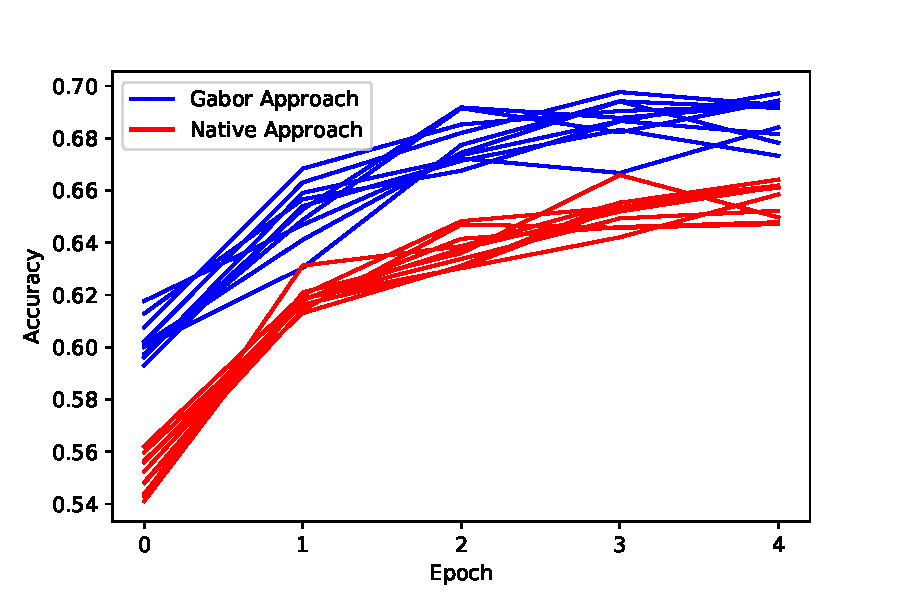
\includegraphics[width=0.7\linewidth]{./papers/visuell/images/accuracy}
	\caption{Test-Genauigkeit (Accuracy) der beiden Varianten im Laufe des Trainings.}
	\label{fig:acc}
\end{figure}

Ein weiterer wichtiger Punkt bei neuronalen Netzen sind die Geschwindigkeiten
Bei der Variante mit Gabor dauerte das Training in etwa 3 Minuten und 10 Sekunden (kann abhängig vom Computer und Grafikkarte stark variieren).
Bei der zweiten Variante, wo erste Layer ebenfalls gelernt wird, dauert das Training ca. 15\% länger (also etwa 3 Minuten und 38 Sekunden).
Das Klassifizieren von neuen Bildern dauert danach bei beiden Varianten gleich lange, da in beiden Fällen die identische Tensorflow-Struktur implementiert wurde.